\documentclass[12pt]{article}

%\usepackage{graphics}
\usepackage{graphicx}
\usepackage{caption}
\usepackage{subcaption}
%\usepackage{epsfig}
%\usepackage{times}
%\usepackage{amsmath}
%\usepackage[spanish]{babel}
%\usepackage{lscape}
%\usepackage[nottoc,numbib]{tocbibind}
%\usepackage{pdfpages}

\title{Exercise 1}
\date{\today}
%\author{Mat\'{\i}as Rivero}

\begin{document}
\maketitle

\section{Assignment}
In engineering, the stresses are one of the prinicipal variables which helps to predict the failure of a mechanical component, defined by a specific shape and material, and subjected to specific boundary conditions. Particular zones in a given mechanical component where stresses ``concentrates'' and tends to infinity in the continumm must be avoided. This stress concentration depends on the shape of the component and special emphasis should be put on this issue during designing process. Finite element analysis helps to predict the stress distribution of a mechanical piece under certain boundary conditions. This is of great help for the engineer during the design process. As the cost of performing a computer simulation of a given mechanical component is low compared with experiments, the engineer has the oportunity to redesign several times a specific component and evaluate its performance until all usage requeriments are fullfiled. 

\medskip

Let's consider an L-shaped beam made of aluminium subjected only to Dirichlet boundary conditions. The geometry, material properties and boundary conditions are given by Fig.~\ref{fig:geometry}.
\begin{itemize}
\item Run this problem using Ostero and postprocess the results with ParaView. 
\item Using ParaView, look for the point of maximum $\sigma_{xx}$ stress (to do this, split horizontally the Layout, create a SpreadSheet View and sort the SIGXX variable).
\item Refine the mesh and see how this value (and position) evolves. To refine the mesh, edit the .geo file and check for the hints. How is the evolution of the maximum value of $\sigma_{xx}$ after refining the mesh several times?
\item Propose a new design to improve this performance. Why the performance you observed in the previous point is undesired?
\item Generate the geometry and mesh of your proposed design and perform a mesh convergence analysis to check the improvement.
\end{itemize}

If you get lost, in the RESOLUTION folder you will find several hints that will help you with the fullfilment of this assignment.

\vspace{2cm}

\begin{figure}[htp]
\begin{center}
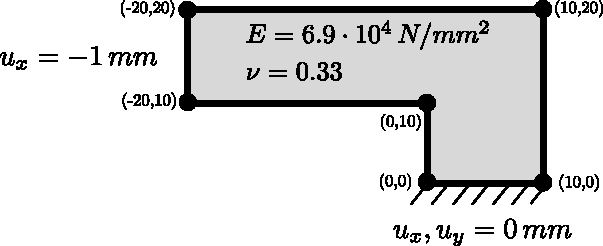
\includegraphics[width=1\linewidth]{Lbeam.pdf}
\caption{Geometry, properties and boundary conditions.}
\label{fig:geometry}
\end{center}
\end{figure}

\vspace{2cm}

\hrulefill


%~\cite{bib:belytschko}.
%\begin{thebibliography}{9}
%\bibitem{bib:belytschko} {\it Nonlinear Finite Elements for Continua and Structures}. Ted Belytschko, Wing Kam Liu, Brian Moran. Wiley, 2000. 
%\end{thebibliography}

\end{document}
